% Created 2020-04-29 Wed 13:38
% Intended LaTeX compiler: pdflatex
\documentclass[11pt]{article}
\usepackage[utf8]{inputenc}
\usepackage[T1]{fontenc}
\usepackage{graphicx}
\usepackage{grffile}
\usepackage{longtable}
\usepackage{wrapfig}
\usepackage{rotating}
\usepackage[normalem]{ulem}
\usepackage{amsmath}
\usepackage{textcomp}
\usepackage{amssymb}
\usepackage{capt-of}
\usepackage{hyperref}
\usepackage{minted}
\usepackage{mdframed}
\BeforeBeginEnvironment{minted}{\begin{mdframed}}
\AfterEndEnvironment{minted}{\end{mdframed}}
\setcounter{secnumdepth}{3}
\author{Karl Gemayel}
\date{Mon 27 Apr 2020 10:37:05 EDT}
\title{Reproducing SBSP\\\medskip
\large The commands used to set up, reproduce, and graph results from the SBSP paper}
\hypersetup{
 pdfauthor={Karl Gemayel},
 pdftitle={Reproducing SBSP},
 pdfkeywords={},
 pdfsubject={},
 pdfcreator={Emacs 26.3 (Org mode 9.3.6)}, 
 pdflang={English}}
\begin{document}

\maketitle
\setcounter{tocdepth}{2}
\tableofcontents


\section{Downloading and installing}
\label{sec:org094ae03}
\subsection{Code}
\label{sec:orgd6446fa}
Downloading the code is fairly straightforward using \texttt{git}.

\subsection{Data}
\label{sec:orgcc1b9e1}
We provide the databases for \emph{Enterobacterales}, \emph{Actinobacteria}, \emph{Archaea}, and \emph{FCB group}, and the sequence and label files for the genomes with verified starts: \emph{E. coli}, \emph{H. salinarum}, \emph{N. pharaonis}, \emph{M. tuberculosis}. We also provide the steps to create a data base with for any ancestor using data that can be downloaded from NCBI's website.

\section{Code and data structure}
\label{sec:org70f89c6}
After installing SBSP, you will have the following structure

\begin{center}
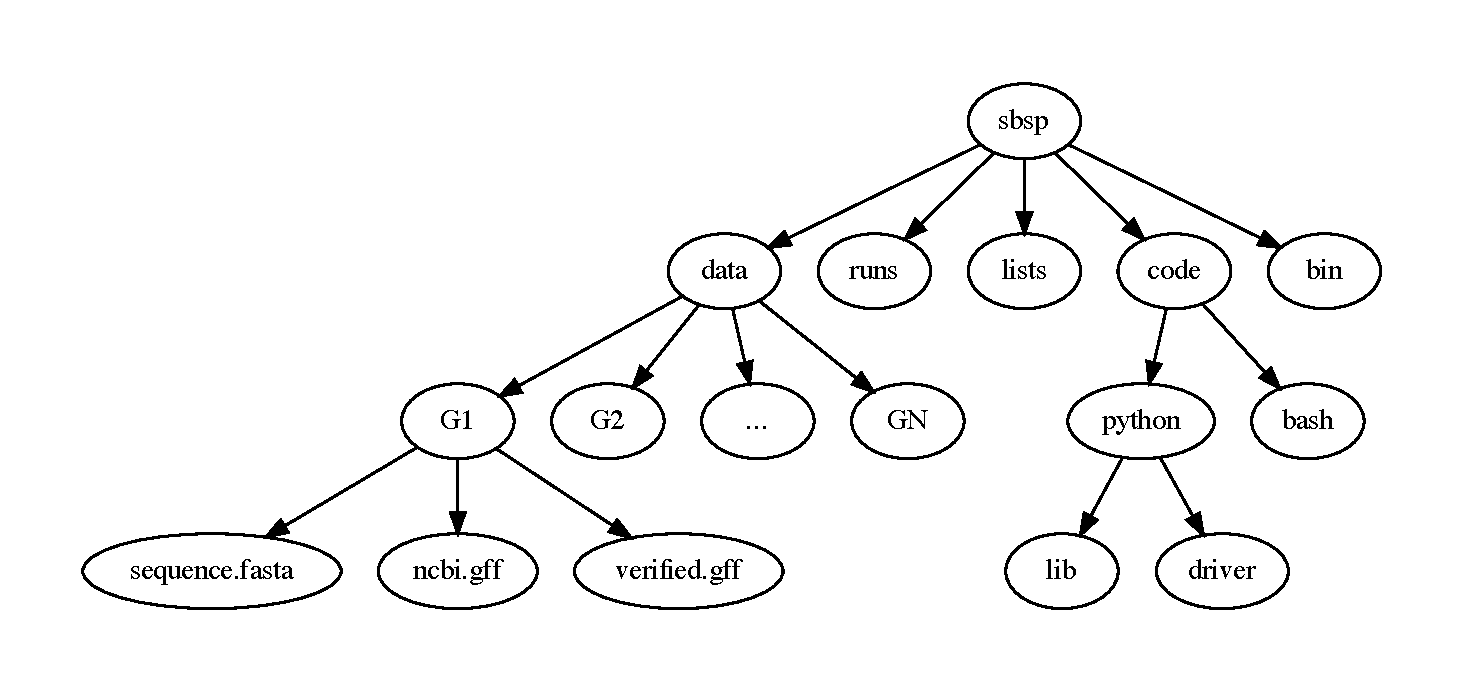
\includegraphics[width=.9\linewidth]{dir.pdf}
\end{center}

\subsection{Bin}
\label{sec:orgb22d4c4}
The python scripts can be located at 
\subsection{Data}
\label{sec:org690cfb3}
The data directory contains all genomic raw information: mainly the sequence and labels files. If constructing databases from scratch, this directory will also include all genomes downloaded from NCBI.
\subsection{Runs}
\label{sec:org0040d12}
For this analysis, all runs executed by SBSP, GMS2, and Prodigal will be put in subdirectories for each genome. 
\begin{center}
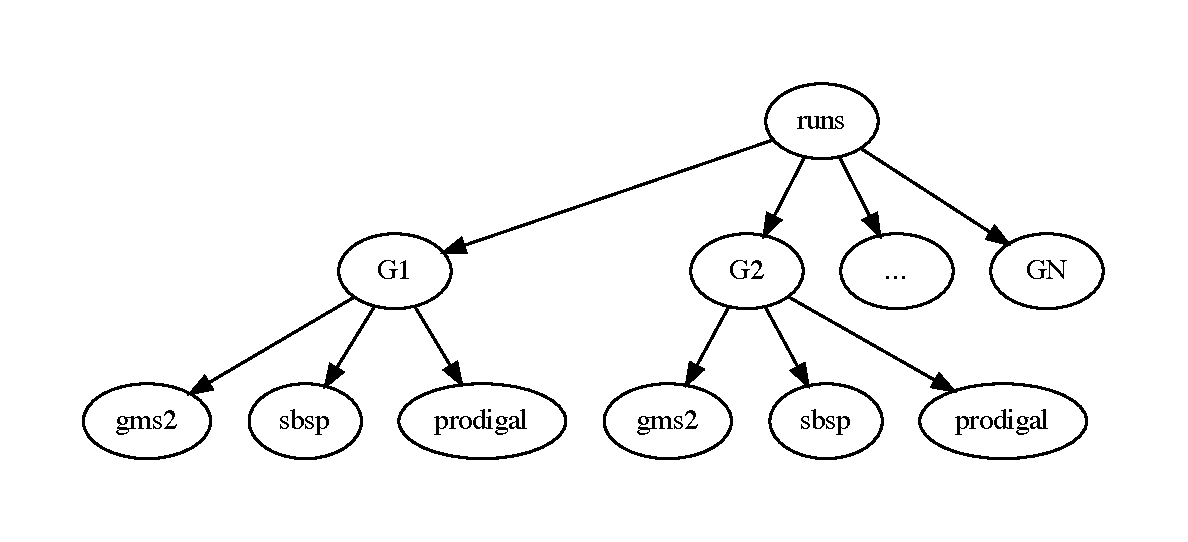
\includegraphics[width=.9\linewidth]{dir_runs.pdf}
\end{center}


\section{Running on verified genomes}
\label{sec:orgc17482e}

SBSP takes as input:
\begin{itemize}
\item Query proteins: FASTA file
\item Target protein database: Diamond database
\end{itemize}

It outputs:
\begin{itemize}
\item GFF file containing labels
\item Multiple sequence alignment files for all queries
\item details.csv: output file containing details of predictions
\end{itemize}



\begin{minted}[breaklines=true,breakanywhere=true,breaksymbolleft=\t,breaksymbolright=\textbackslash]{bash}
# List of genomes with verified genes
pf_list_verified=$lists/verified.list
pf_sbsp_conf=$config/sbsp_defaults.conf

toggle_pbs="--pf-conf-pbs $config/pbs_defaults.conf"  # if PBS installed, set this option to empty: ""

$bin/run_sbsp_from_genome_list_py.sh --pf-genome-list ${pf_list_verified} --pf-conf-sbsp ${pf_sbsp_conf} ${toggle_pbs} 

\end{minted}

\section{GMS2 on metagenomes}
\label{sec:orgc561bb0}
\subsection{Run GMS2 on genome fragments}
\label{sec:org3a5020c}
\begin{minted}[breaklines=true,breakanywhere=true,breaksymbolleft=\t,breaksymbolright=\textbackslash]{bash}
$bin/analysis_on_genome_fragments_py.sh --pf-genome-list $lists/verified.list --tools gms2 prodigal
\end{minted}
\section{Collecting Data}
\label{sec:orga716c8d}

\section{Tables and Graphs}
\label{sec:org1765fc9}
\subsection{}
\label{sec:org73bd545}
\end{document}
